\subsubsection{General Route}
In this model, we estimate the overall positive impact of a many-to-many alliance to one ally.

When a customer does a purchase in an ally, he receives \RPd s for the alliance. Then he will browse where he can use them for a discount. This gives a chance of advertisement for every ally in the alliance.
But at the meantime, if an ally is not famous, when a customer views the list of allies in the alliance, the customer may ignore the ally and focus his attention on those famous allies.
The former positive impact is called \textsl{Advertising Impact} ($I_A$) while the latter negative \textsl{Drowning Impact} ($I_D$).

In a given limited area, the higher the $RC$, the more likely customers living in the area will see the advertisement, so the higher the overall positive impact. The product type overlap also plays a role. So:
\[  I = \Phi \cdot RC \cdot (I_A - I_D)  \]

\subsubsection{Cover Rate}
We take the area containing all the merchants in the alliance as the total area. As the merchants join the alliance, the area covered by new merchants overlaps with the already covered area. Generally, the later the merchant joins, the more its area overlaps with the already covered, and the less new area it covers. Therefore, as the number of merchants rise, the covered area shows a \textsl{Diminishing Marginal Returns}.

The first task is to decide the total area by the location of the allies. We draw some points on the map, representing the merchants. We connect each two and will get a closed figure. Since $r=200m$, we expand the whole figure by $400m$. That is the final total area. An example is shown in Figure \ref{fig:total_area}.

\begin{figure}[H]
	\centering
	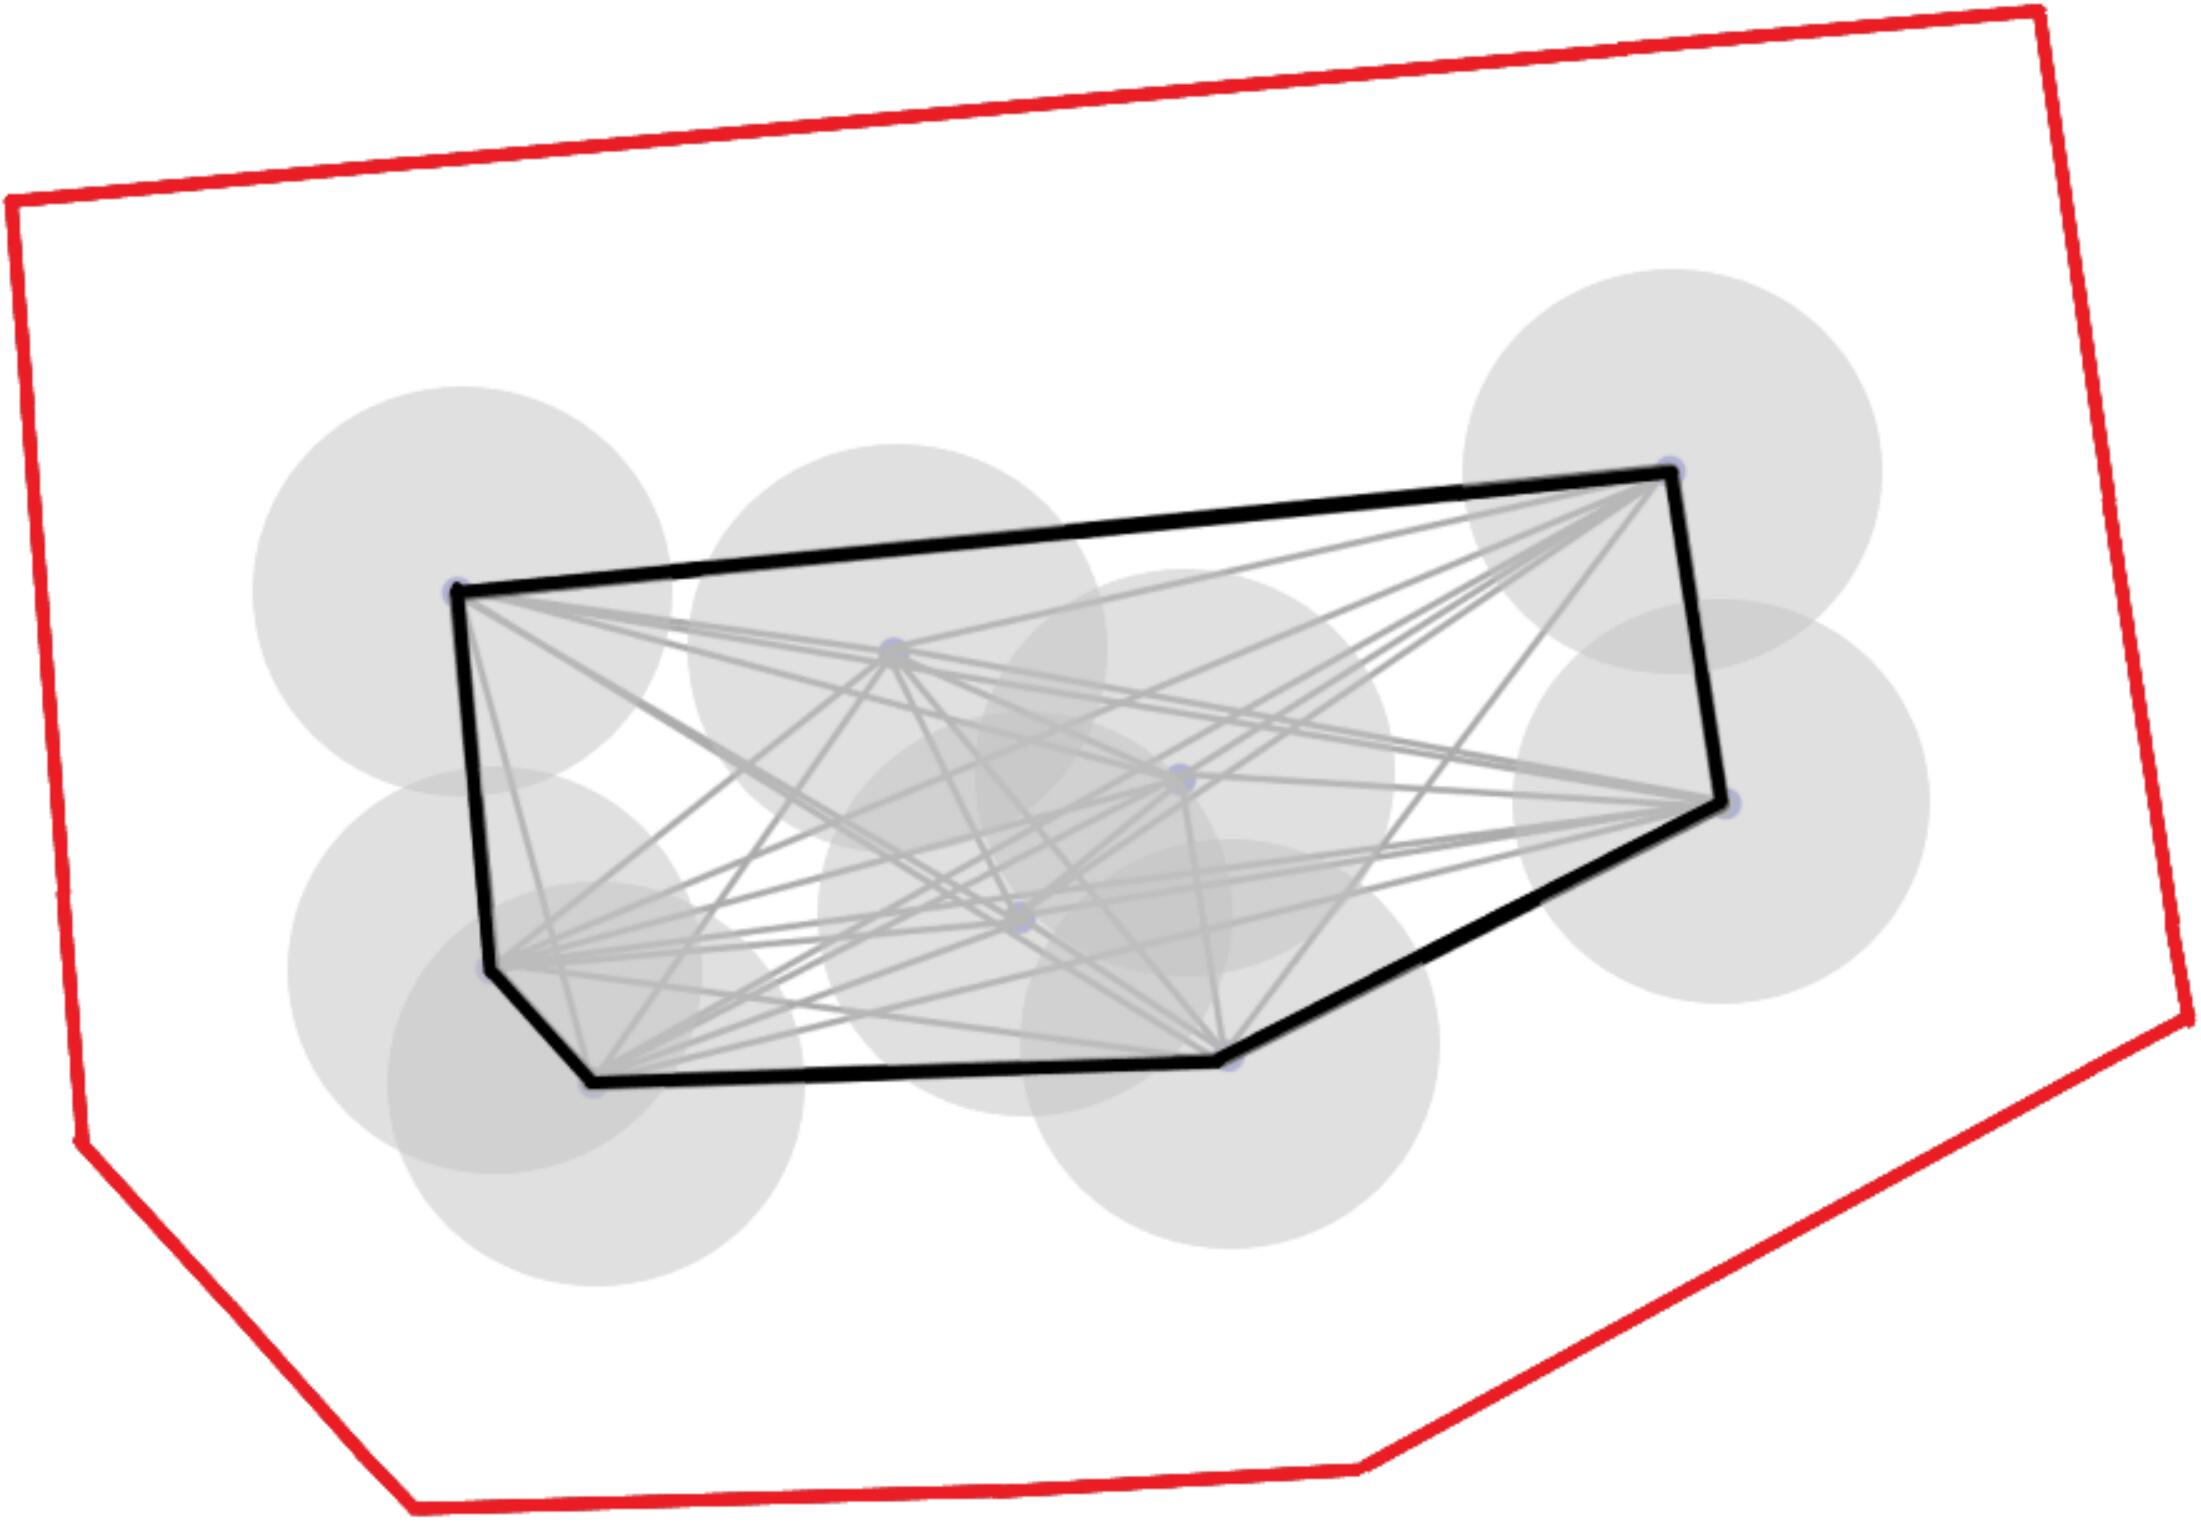
\includegraphics[width=9cm]{total_area.jpg}
	\caption{an example of the calculation of the total area}
	\label{fig:total_area}
\end{figure}

After going through an amount of residential and merchant areas, we can safely suppose that the distance from resident areas to the nearest merchant is within two times the radius of the coverage circle. The thin black lines connect each 2 merchants. The bold lines are the outermost lines and they form a polygon. Since the residential area usually appears to be like rectangles, we draw lines parallel with each side outside the polygon. These lines are connected to form the red line, which shows the total area border.

What we need to do is developing $RC=f(n)$. Obviously,
\[  \begin{cases}
f(0) = 0 \\
\frac{d}{dn} RC > 0 \\
0 \le RC < 1 \\
\frac{d}{d^2n} RC^2 < 0
\end{cases}  \]

Two common functions fit the requirements:
$ f(n) = \frac{n}{n+k} $ and $ f(n) = -k^n+1 $.
We search for some typical places where there are merchants among several residential areas. By \textit{Monte Carlo} method, we calculate several $(n,RC)$ and get the best $k$ and the best function through curve fitting.

\[f(n) = -k^n+1\]

Coefficients (with 95\% confidence bounds):
\[k = 0.8305  (0.8182, 0.8429)\]

\begin{center}
Goodness of fit:

  SSE: 0.002902
  
  R-square: 0.9912
  
  Adjusted R-square: 0.9912
  
  RMSE: 0.02409
\end{center}

\begin{figure}[H]
	\centering
	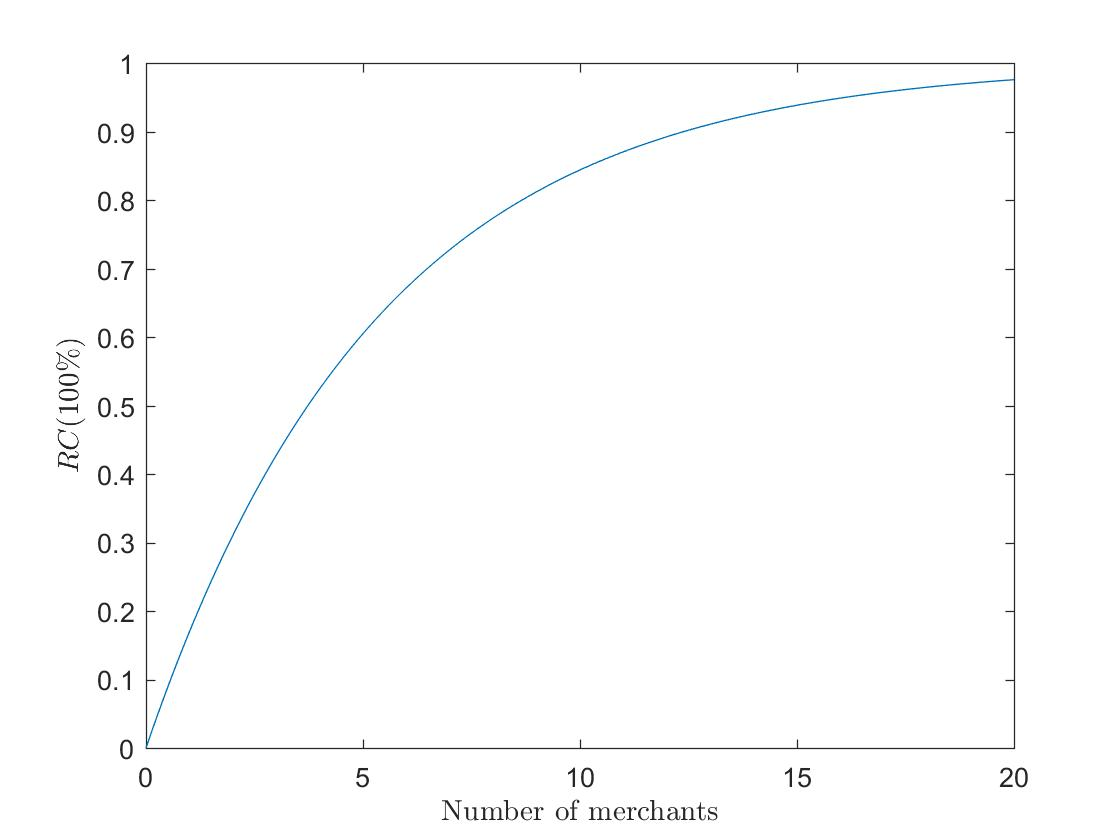
\includegraphics[width=10.5cm]{RC_function.jpg}
	\caption{the image of function RC=f(n)}
	\label{fig:RC_function}
\end{figure}

\subsubsection{Advertising Impact}
The $I_A$, as its name indicates, has a linear relationship with the times an ally is advertised. Hence, $I_A \propto (n-1)$. So we consider
\[  I_A = k_A (n-1)  \]
in which $k_A$ is a constant that will be measured later.

\subsubsection{Drowning Impact}
The $I_D$ is straightly related to the scale of the ally and the scale sum of all allies in the alliance.

The higher the reputation of an ally in the alliance, the less it will suffer from the \textsl{Drowning Effect}.

Suppose
\[  s = \frac{s_X}{\overline{s}} 
= \frac{n \cdot s_x}{\sum\limits_{i=1}^n S_i}  \]

So,
\[
I_D \propto
\frac{\textup{the total scale of the alliance}}{\textup{the relative scale of the ally}}
=
\frac{u(s_1,s_2,\ldots,s_n)}{v(s)}
\]

Obviously, the relationship between $s$ and $I_D$ is not linear. It should fit in with
\[\begin{cases}
\frac{d}{ds} I_D < 0 \\
\frac{d}{d^2s} {I_D}^2 > 0 \\
\forall i,j \in \{1,2,\ldots,n\}, S_i < S_j,
\frac{\partial u}{\partial S_i} < \frac{\partial u}{\partial S_j}
\end{cases}\]

By calculating with calculus, we find a suitable answer.
\[
u(s_1,s_2,\ldots,s_n) = \sum\limits_{i=1}^n {s_i}^2
\]

\[  v(s) = e^x  \]

So for the $I_D$, as is shown in figure \ref{fig:drowning_effect},
\[  I_D = \frac{\sum\limits_{i=1}^n {s_i}^2}{e^s}  \]
\begin{figure}[H]
\centering
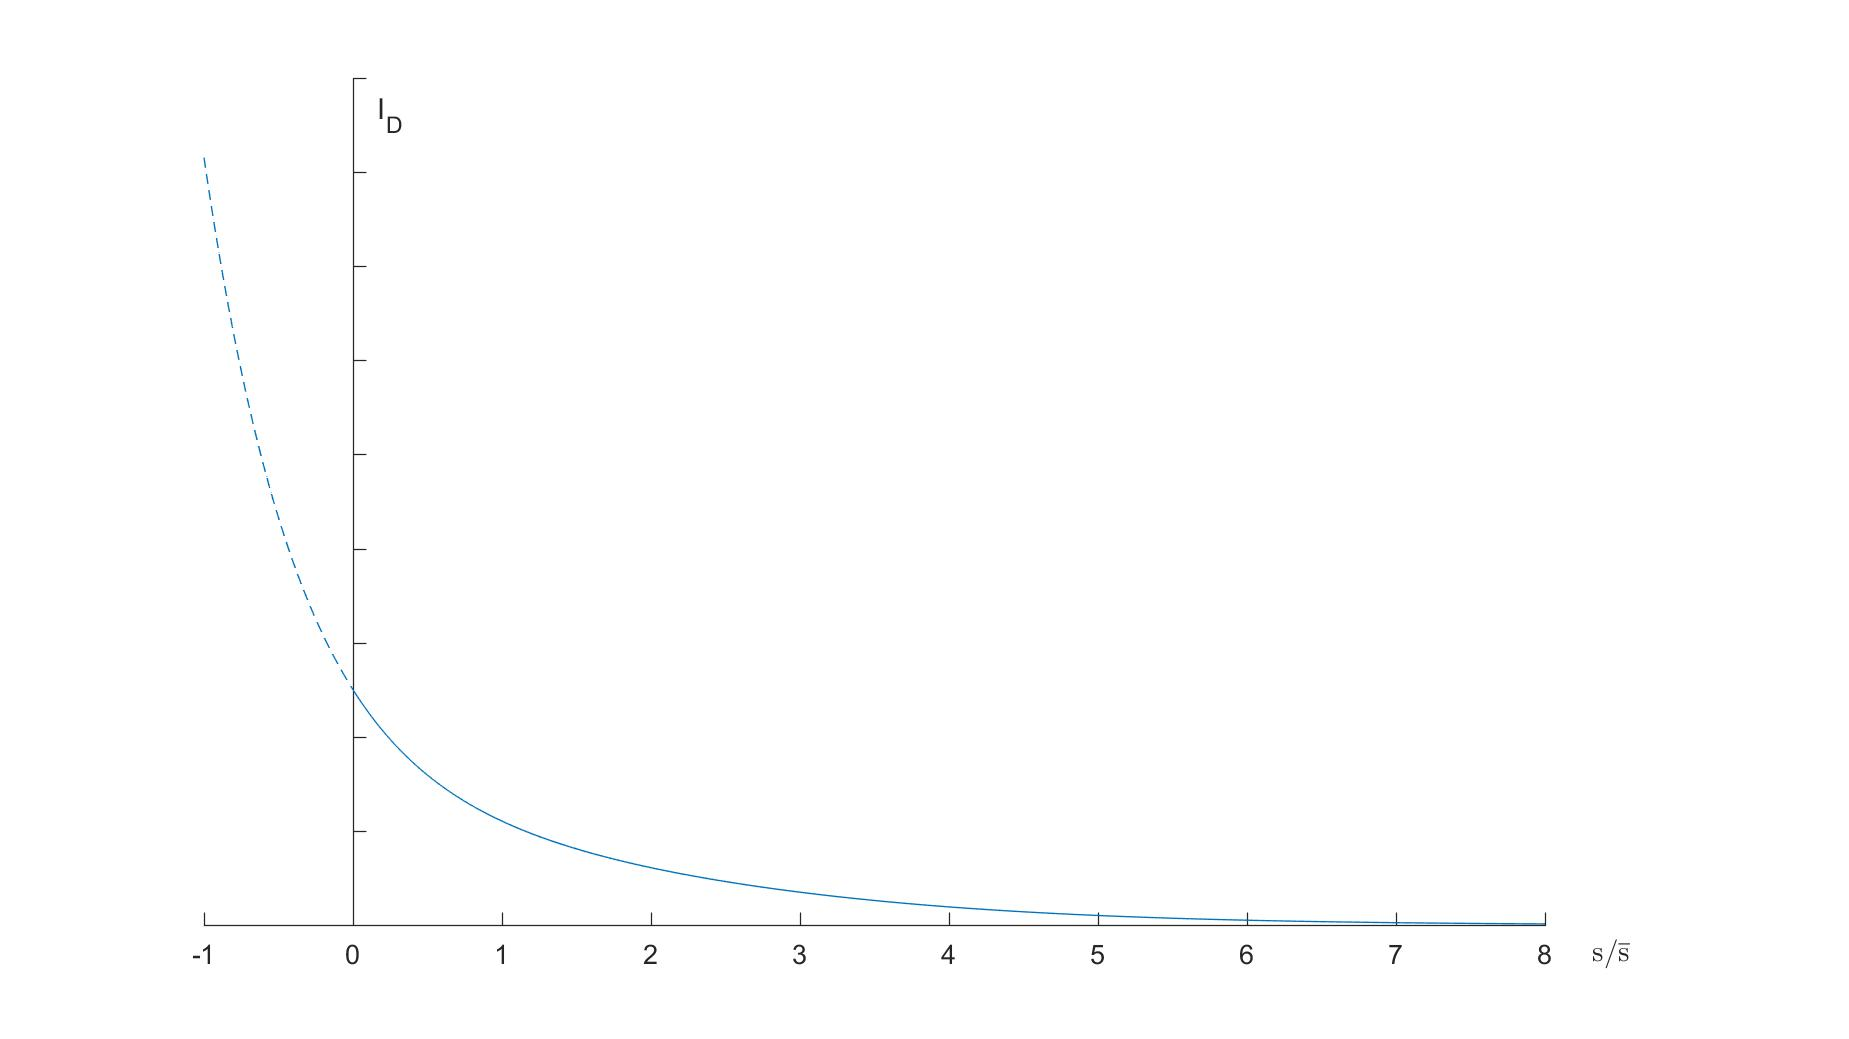
\includegraphics[width=0.7\linewidth]{drowning_effect.jpg}
\caption{the relationship between relative $I_D$ and scale of the ally}
\label{fig:drowning_effect}
\end{figure}

\begin{figure}[H]
\centering
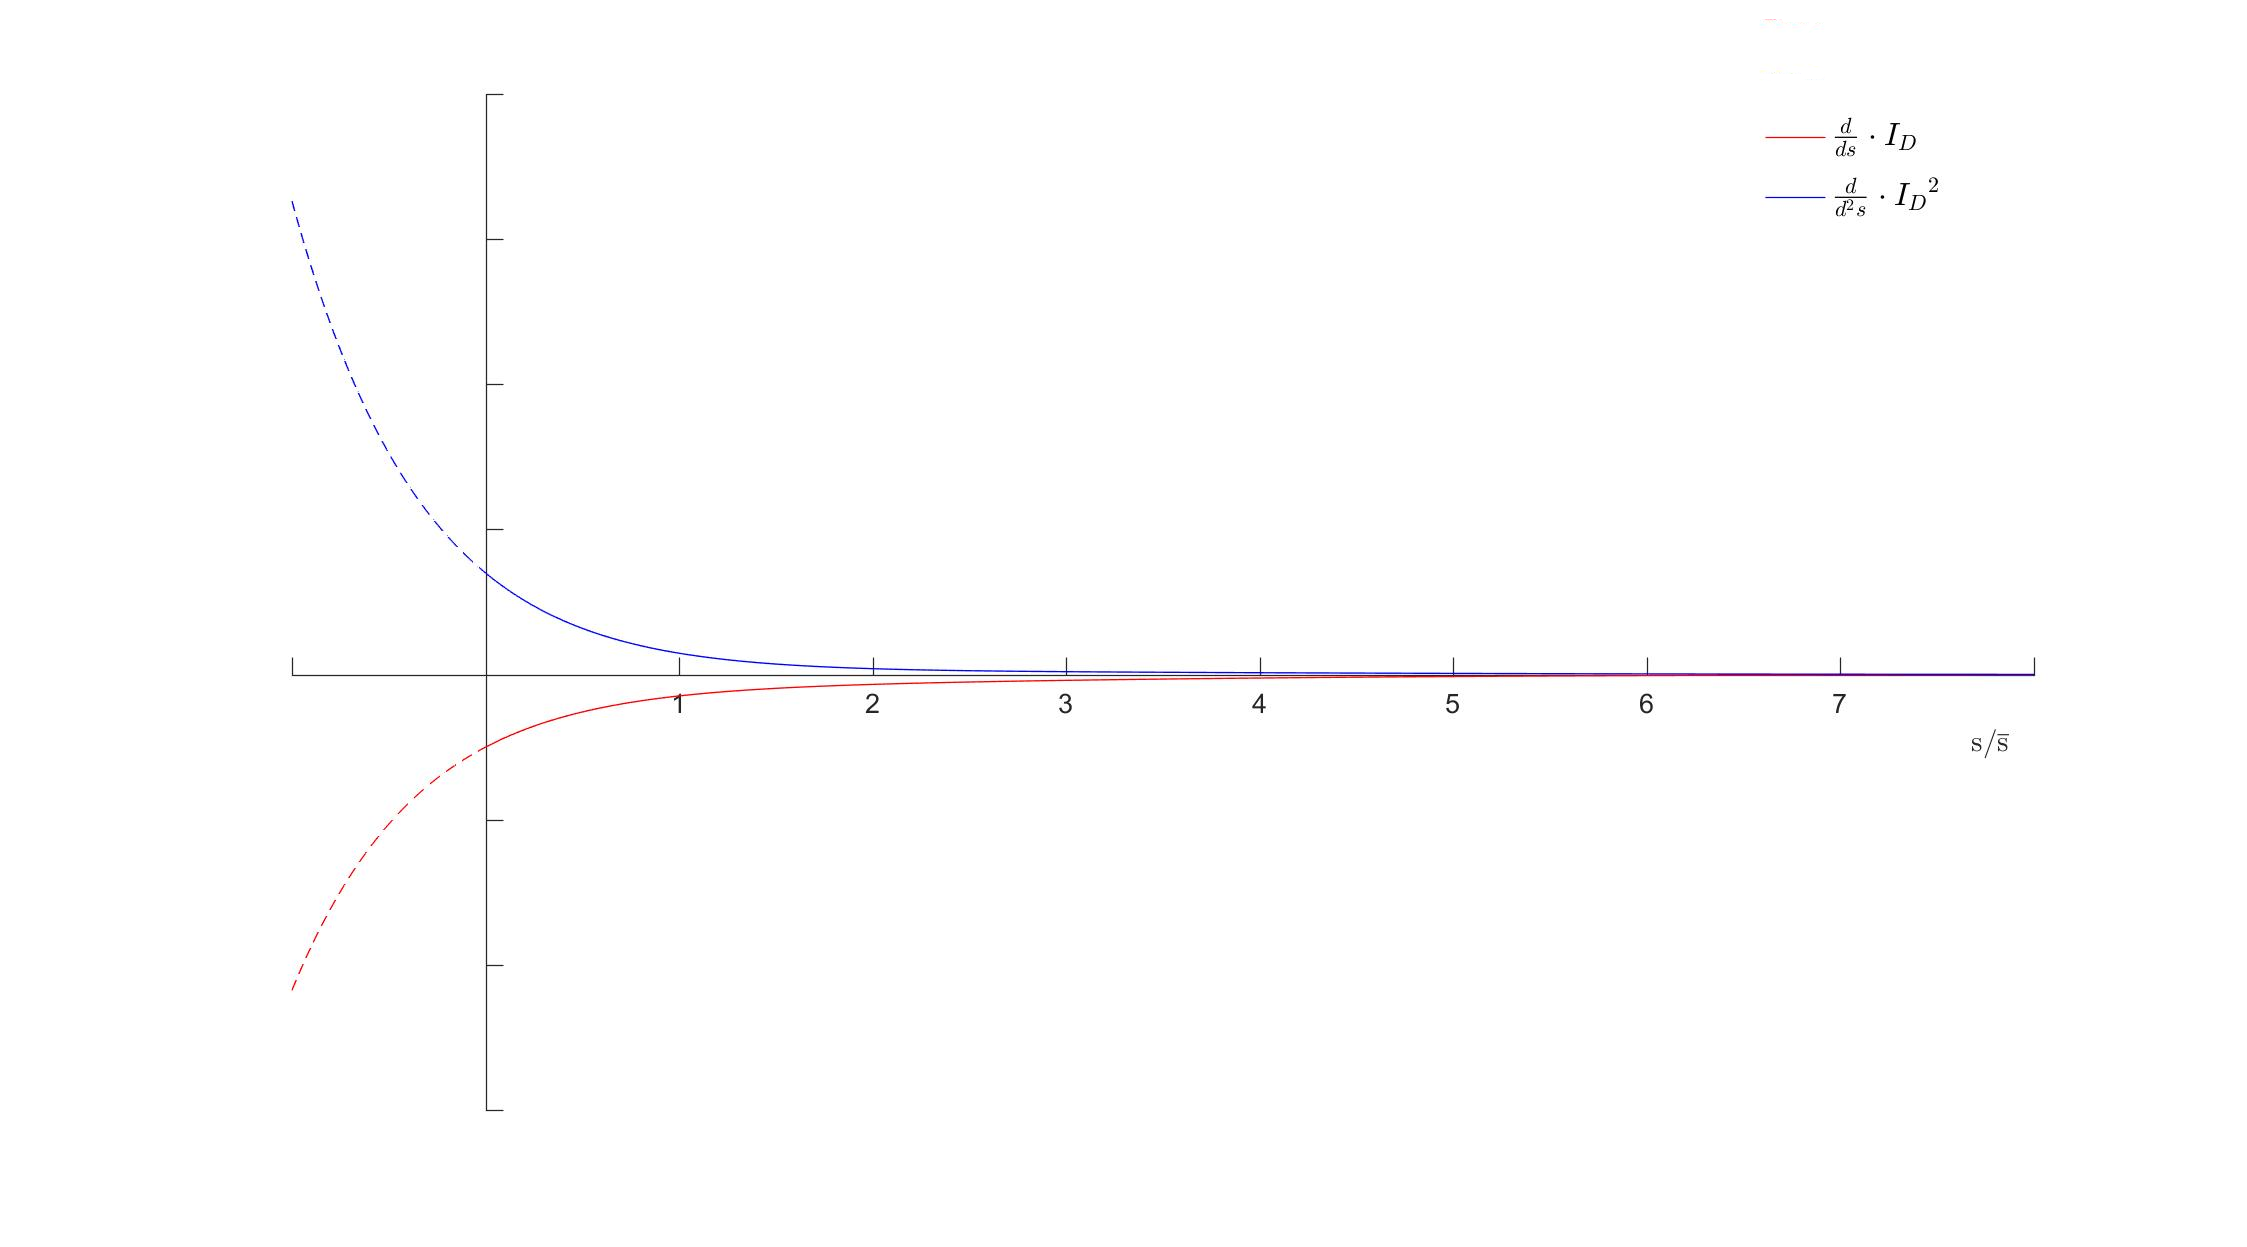
\includegraphics[width=0.7\linewidth]{drowning_effect_calculus.png}
\caption{the features of the relationship between relative $I_D$ and scale of the ally}
\label{fig:drowning_effect_calculus}
\end{figure}

\subsubsection{Product Type}
We decompose the overall impact of product type on \X{X}\ ($\Phi_X$) into several sub-impact for every product type.

Let us make our object the impact from product type of \B\ to \A. Then we calculate the overlapping rate of each column (universal product type classification).
\[  \phi_{i,B} = 
\frac{\sum_{\begin{subarray}{c}
\textup{for each overlapping} \\ \textup{Product}\ i
\end{subarray}} P_i}%
{\sum_{\begin{subarray}{c}
\textup{for each } \\ \textup{Product}\ j
\end{subarray}} P_j}  \]

\[  \phi_B = \sum\limits_{i=1}^{M_i} \phi_{i,B}  \]

Here is an example of the calculation of $\phi$. Its final result is $\Phi=171\%$.

\begin{table}[H]
\begin{tabular}{|c|p{.7\textwidth}|c|}
\hline
Product Type & Products & $\phi_{i,B}$ \\
\hline
Dishwasher & \tabincell{l}{(A) \$359.99, \$350.00 \\ (B) \$349.00, \$330.00 \\ (A\&B) \$512.80, \$399.99} & 39.7\% \\
\hline
Microwave Oven & \tabincell{l}{(A) \$99.98, \$212.40 \\ (B) \$59.98, \$95.30, \$111.99 \\ (A\&B) \$96.67, \$134.99} & 28.6\% \\
\hline
Refrigerator & \tabincell{l}{(A) \$783.19, \$511.40 \\ (B) \$599.00, \$872.02 \\ (A\&B) \$279.00, \$635.33} & 24.8\% \\
\hline
Laundry & \tabincell{l}{(A) \$205.99, \$279.99 \\ (B) \$163.99 \\ (A\&B) \$253.33, \$249.99, \$323.51} & 56.0\% \\
\hline
Range Hood & \tabincell{l}{(A) \$323.82, \$382.21 \\ (B) \$359.26, \$290.91, \$284.99 \\ (A\&B) \$459.96} & 21.9\% \\
\hline
\end{tabular}
\caption{an example of the calculation of $\phi$}
\label{tab:phi_calc}
\end{table}

Now the last problem is how to sum up the impact of each ally to the merchant. By market experience, one suitable relationship between $\phi_X$ and $\Phi_{X}$ is
\[  \Phi_{X} = {\sum_{X=1}^{n-1} \phi_X}  \]
\[  = {\sum_{X=1}^{n-1} {\sum\limits_{i=1}^{M_i} \phi_{i,X}}}  \]

\subsubsection{Overall Algorithm}
For a certain ally,
\[  I = \Phi \cdot RC \cdot (I_A - I_D)  \]
\[  = {\sum_{X=1}^{n-1} \phi_X} \cdot (-0.8305^n+1) \cdot \left[k_A (n-1) - \frac{\sum_{i=1}^n {s_i}^2}{e^s}\right]   \]
\[  = {\sum_{X=1}^{n-1} {\sum\limits_{i=1}^{M_i} \phi_{i,X}}} \cdot (-0.8305^n+1) \cdot \left[k_A (n-1) - \frac{\sum_{i=1}^n {s_i}^2}{e^s}\right]  \]

The relative importance will be further discussed in the section \textsl{Sensitivity Analysis}.

Then we test the model result. We get the value of the constant $k_A=50$ and make a modification to modify $I$'s order of magnitude. The final result is
\begin{equation}
I = \left({\sum_{X=1}^{n-1} {\sum_{i=1}^{M_i} \phi_{i,X}}} \cdot (-0.8305^n+1) \cdot \left[50(n-1) - \frac{\sum_{i=1}^n {s_i}^2}{e^{\sqrt{s}}}\right]\right)^\frac{1}{3}
\label{eq:mtm_model}
\end{equation}
